% IEEEtran conference paper (draft, Gun 17). Turkish text, English abstract and index terms.
% Every number in running text is a macro from numbers.tex (generated from reports/ by
% scripts/make_paper_numbers.py); the tables in tables/*.tex are generated by scripts/make_tables.py.
% Compile on Overleaf (IEEEtran is built in): main.tex + numbers.tex + refs.bib + tables/ + figures/.
\documentclass[conference]{IEEEtran}
\IEEEoverridecommandlockouts

\usepackage[utf8]{inputenc}
\usepackage[T1]{fontenc}
\usepackage[turkish]{babel}
\usepackage{amsmath,amssymb}
\usepackage{booktabs,array}
\usepackage{graphicx}
\usepackage{textcomp}
\usepackage{cite}
\usepackage{url}
\usepackage{xcolor}

% characters that appear in the generated tables (scripts/make_tables.py)
\DeclareUnicodeCharacter{03B4}{\ensuremath{\delta}}
\DeclareUnicodeCharacter{03B8}{\ensuremath{\theta}}
\DeclareUnicodeCharacter{2212}{\ensuremath{-}}

% Generated by scripts/make_paper_numbers.py from reports/tables: DO NOT EDIT BY HAND.
% Each macro is one cell (or one documented derivation) of a results file; see NUMBERS.md.
\newcommand{\nSeed}{42}
\newcommand{\nOptunaTrials}{20}
\newcommand{\nExtremeQuantilePct}{95}
\newcommand{\nWaitMs}{500}
\newcommand{\nCooldownH}{6}
\newcommand{\nBeta}{2}
\newcommand{\nThetaLow}{75}
\newcommand{\nThetaHigh}{150}
\newcommand{\nSpeedSlow}{3600}
\newcommand{\nSpeedFast}{36000}
\newcommand{\nReps}{3}
\newcommand{\nFfillLimit}{3}
\newcommand{\nHazeMinStations}{8}
\newcommand{\nHazeMinHours}{6}
\newcommand{\nEventMinHours}{3}
\newcommand{\nEventMergeGapH}{6}
\newcommand{\nWarnWindowH}{24}
\newcommand{\nQuantLow}{0.1}
\newcommand{\nQuantMid}{0.5}
\newcommand{\nQuantHigh}{0.9}
\newcommand{\nKThree}{3}
\newcommand{\nKEleven}{11}
\newcommand{\nSimDays}{14}
\newcommand{\nTargetCoverage}{0.80}
\newcommand{\nCpuCount}{12}
\newcommand{\nRamGb}{17}
\newcommand{\nPyVersion}{3.11.9}
\newcommand{\nBrokerVersion}{2.1.4}
\newcommand{\nDataRows}{420768}
\newcommand{\nDataHours}{35064}
\newcommand{\nDataMissingPct}{2.08}
\newcommand{\nDataMean}{79.8}
\newcommand{\nDataPNinetyFive}{242}
\newcommand{\nPmInconsistentTrainPct}{8.2}
\newcommand{\nDataStations}{12}
\newcommand{\nTrainStart}{2013-03}
\newcommand{\nTrainEnd}{2015-08}
\newcommand{\nValStart}{2015-09}
\newcommand{\nValEnd}{2016-02}
\newcommand{\nTestStart}{2016-03}
\newcommand{\nTestEnd}{2017-02}
\newcommand{\nEventsHaze}{43}
\newcommand{\nEventsFifty}{1467}
\newcommand{\nEventsHundred}{724}
\newcommand{\nRmsePersistHOne}{19.65}
\newcommand{\nRTwoPersistHOne}{0.94}
\newcommand{\nImprPersistHOne}{0.0}
\newcommand{\nRmsePersistHSix}{54.88}
\newcommand{\nRTwoPersistHSix}{0.56}
\newcommand{\nImprPersistHSix}{0.0}
\newcommand{\nRmsePersistHTwentyFour}{88.12}
\newcommand{\nRTwoPersistHTwentyFour}{-0.13}
\newcommand{\nImprPersistHTwentyFour}{0.0}
\newcommand{\nRmseSeasonalHOne}{88.14}
\newcommand{\nRTwoSeasonalHOne}{-0.13}
\newcommand{\nImprSeasonalHOne}{-348.6}
\newcommand{\nRmseSeasonalHSix}{88.16}
\newcommand{\nRTwoSeasonalHSix}{-0.13}
\newcommand{\nImprSeasonalHSix}{-60.6}
\newcommand{\nRmseSeasonalHTwentyFour}{88.12}
\newcommand{\nRTwoSeasonalHTwentyFour}{-0.13}
\newcommand{\nImprSeasonalHTwentyFour}{0.0}
\newcommand{\nRmseRidgeHOne}{18.54}
\newcommand{\nRTwoRidgeHOne}{0.95}
\newcommand{\nImprRidgeHOne}{5.6}
\newcommand{\nRmseRidgeHSix}{50.05}
\newcommand{\nRTwoRidgeHSix}{0.64}
\newcommand{\nImprRidgeHSix}{8.8}
\newcommand{\nRmseRidgeHTwentyFour}{73.66}
\newcommand{\nRTwoRidgeHTwentyFour}{0.21}
\newcommand{\nImprRidgeHTwentyFour}{16.4}
\newcommand{\nRmseMoneHOne}{17.85}
\newcommand{\nRTwoMoneHOne}{0.95}
\newcommand{\nImprMoneHOne}{9.1}
\newcommand{\nRmseMoneHSix}{48.88}
\newcommand{\nRTwoMoneHSix}{0.65}
\newcommand{\nImprMoneHSix}{10.9}
\newcommand{\nRmseMoneHTwentyFour}{73.53}
\newcommand{\nRTwoMoneHTwentyFour}{0.21}
\newcommand{\nImprMoneHTwentyFour}{16.6}
\newcommand{\nRmseMtwoaHOne}{16.99}
\newcommand{\nRTwoMtwoaHOne}{0.96}
\newcommand{\nImprMtwoaHOne}{13.5}
\newcommand{\nRmseMtwoaHSix}{47.89}
\newcommand{\nRTwoMtwoaHSix}{0.67}
\newcommand{\nImprMtwoaHSix}{12.7}
\newcommand{\nRmseMtwoaHTwentyFour}{73.35}
\newcommand{\nRTwoMtwoaHTwentyFour}{0.22}
\newcommand{\nImprMtwoaHTwentyFour}{16.8}
\newcommand{\nRmseMtwobHOne}{17.08}
\newcommand{\nRTwoMtwobHOne}{0.96}
\newcommand{\nImprMtwobHOne}{13.1}
\newcommand{\nRmseMtwobHSix}{46.60}
\newcommand{\nRTwoMtwobHSix}{0.68}
\newcommand{\nImprMtwobHSix}{15.1}
\newcommand{\nRmseMtwobHTwentyFour}{73.29}
\newcommand{\nRTwoMtwobHTwentyFour}{0.22}
\newcommand{\nImprMtwobHTwentyFour}{16.8}
\newcommand{\nImprMtwobCiLoHOne}{9.9}
\newcommand{\nImprMtwobCiHiHOne}{16.2}
\newcommand{\nSigMtwobHOne}{12/12}
\newcommand{\nAblKthreeHOne}{4.8}
\newcommand{\nAblKthreeSigHOne}{10/12}
\newcommand{\nAblKelevenHOne}{4.3}
\newcommand{\nAblKelevenSigHOne}{10/12}
\newcommand{\nLosoMeanHOne}{12.6}
\newcommand{\nLosoInSampleHOne}{13.1}
\newcommand{\nLosoBetterHOne}{12}
\newcommand{\nDmMtwobVsBZeroHOne}{12}
\newcommand{\nDmMtwobVsMOneHOne}{10}
\newcommand{\nShapLagZeroHOne}{43.1}
\newcommand{\nShapNbMeanHOne}{6.3}
\newcommand{\nExtRmsePersistHOne}{40.5}
\newcommand{\nExtBiasPersistHOne}{6}
\newcommand{\nExtRmseMtwobHOne}{41.4}
\newcommand{\nExtBiasMtwobHOne}{12}
\newcommand{\nImprMtwobCiLoHSix}{10.5}
\newcommand{\nImprMtwobCiHiHSix}{19.6}
\newcommand{\nSigMtwobHSix}{12/12}
\newcommand{\nAblKthreeHSix}{2.0}
\newcommand{\nAblKthreeSigHSix}{5/12}
\newcommand{\nAblKelevenHSix}{4.7}
\newcommand{\nAblKelevenSigHSix}{12/12}
\newcommand{\nLosoMeanHSix}{14.5}
\newcommand{\nLosoInSampleHSix}{15.1}
\newcommand{\nLosoBetterHSix}{12}
\newcommand{\nDmMtwobVsBZeroHSix}{12}
\newcommand{\nDmMtwobVsMOneHSix}{12}
\newcommand{\nShapLagZeroHSix}{15.3}
\newcommand{\nShapNbMeanHSix}{13.8}
\newcommand{\nExtRmsePersistHSix}{117.2}
\newcommand{\nExtBiasPersistHSix}{47}
\newcommand{\nExtRmseMtwobHSix}{124.4}
\newcommand{\nExtBiasMtwobHSix}{91}
\newcommand{\nImprMtwobCiLoHTwentyFour}{7.3}
\newcommand{\nImprMtwobCiHiHTwentyFour}{25.1}
\newcommand{\nSigMtwobHTwentyFour}{12/12}
\newcommand{\nAblKthreeHTwentyFour}{0.3}
\newcommand{\nAblKthreeSigHTwentyFour}{0/12}
\newcommand{\nAblKelevenHTwentyFour}{0.3}
\newcommand{\nAblKelevenSigHTwentyFour}{0/12}
\newcommand{\nLosoMeanHTwentyFour}{17.0}
\newcommand{\nLosoInSampleHTwentyFour}{17.0}
\newcommand{\nLosoBetterHTwentyFour}{12}
\newcommand{\nDmMtwobVsBZeroHTwentyFour}{12}
\newcommand{\nDmMtwobVsMOneHTwentyFour}{0}
\newcommand{\nShapLagZeroHTwentyFour}{8.8}
\newcommand{\nShapNbMeanHTwentyFour}{5.0}
\newcommand{\nExtRmsePersistHTwentyFour}{171.1}
\newcommand{\nExtBiasPersistHTwentyFour}{112}
\newcommand{\nExtRmseMtwobHTwentyFour}{216.3}
\newcommand{\nExtBiasMtwobHTwentyFour}{193}
\newcommand{\nExtPNinetyFive}{232}
\newcommand{\nLosoStations}{12}
\newcommand{\nNowcastRmse}{22.1}
\newcommand{\nTuneGainTenTwenty}{0.5}
\newcommand{\nWarnPrecPersistHOne}{0.817}
\newcommand{\nWarnRecPersistHOne}{0.963}
\newcommand{\nWarnFtwoPersistHOne}{0.930}
\newcommand{\nWarnFaPersistHOne}{0.094}
\newcommand{\nWarnEvRecPersistHOne}{1.000}
\newcommand{\nWarnMEvRecPersistHOne}{0.72}
\newcommand{\nWarnLeadPersistHOne}{7}
\newcommand{\nWarnMLeadPersistHOne}{0}
\newcommand{\nWarnDeltaPersistHOne}{15}
\newcommand{\nHazeCaughtPersistHOne}{43}
\newcommand{\nWarnPrecPersistHSix}{0.530}
\newcommand{\nWarnRecPersistHSix}{0.856}
\newcommand{\nWarnFtwoPersistHSix}{0.762}
\newcommand{\nWarnFaPersistHSix}{0.218}
\newcommand{\nWarnEvRecPersistHSix}{1.000}
\newcommand{\nWarnMEvRecPersistHSix}{0.83}
\newcommand{\nWarnLeadPersistHSix}{16}
\newcommand{\nWarnMLeadPersistHSix}{3}
\newcommand{\nWarnDeltaPersistHSix}{40}
\newcommand{\nHazeCaughtPersistHSix}{43}
\newcommand{\nWarnPrecPersistHTwentyFour}{0.378}
\newcommand{\nWarnRecPersistHTwentyFour}{0.613}
\newcommand{\nWarnFtwoPersistHTwentyFour}{0.545}
\newcommand{\nWarnFaPersistHTwentyFour}{0.218}
\newcommand{\nWarnEvRecPersistHTwentyFour}{1.000}
\newcommand{\nWarnMEvRecPersistHTwentyFour}{0.63}
\newcommand{\nWarnLeadPersistHTwentyFour}{16}
\newcommand{\nWarnMLeadPersistHTwentyFour}{20}
\newcommand{\nWarnDeltaPersistHTwentyFour}{40}
\newcommand{\nHazeCaughtPersistHTwentyFour}{43}
\newcommand{\nWarnEvRecPersistHAny}{1.000}
\newcommand{\nWarnPrecMtwobHOne}{0.865}
\newcommand{\nWarnRecMtwobHOne}{0.955}
\newcommand{\nWarnFtwoMtwobHOne}{0.936}
\newcommand{\nWarnFaMtwobHOne}{0.070}
\newcommand{\nWarnEvRecMtwobHOne}{0.979}
\newcommand{\nWarnMEvRecMtwobHOne}{0.66}
\newcommand{\nWarnLeadMtwobHOne}{5}
\newcommand{\nWarnMLeadMtwobHOne}{1}
\newcommand{\nWarnDeltaMtwobHOne}{10}
\newcommand{\nHazeCaughtMtwobHOne}{43}
\newcommand{\nWarnPrecMtwobHSix}{0.568}
\newcommand{\nWarnRecMtwobHSix}{0.876}
\newcommand{\nWarnFtwoMtwobHSix}{0.790}
\newcommand{\nWarnFaMtwobHSix}{0.181}
\newcommand{\nWarnEvRecMtwobHSix}{0.964}
\newcommand{\nWarnMEvRecMtwobHSix}{0.80}
\newcommand{\nWarnLeadMtwobHSix}{15}
\newcommand{\nWarnMLeadMtwobHSix}{3}
\newcommand{\nWarnDeltaMtwobHSix}{40}
\newcommand{\nHazeCaughtMtwobHSix}{43}
\newcommand{\nWarnPrecMtwobHTwentyFour}{0.482}
\newcommand{\nWarnRecMtwobHTwentyFour}{0.528}
\newcommand{\nWarnFtwoMtwobHTwentyFour}{0.518}
\newcommand{\nWarnFaMtwobHTwentyFour}{0.173}
\newcommand{\nWarnEvRecMtwobHTwentyFour}{0.729}
\newcommand{\nWarnMEvRecMtwobHTwentyFour}{0.52}
\newcommand{\nWarnLeadMtwobHTwentyFour}{19}
\newcommand{\nWarnMLeadMtwobHTwentyFour}{21}
\newcommand{\nWarnDeltaMtwobHTwentyFour}{40}
\newcommand{\nHazeCaughtMtwobHTwentyFour}{39}
\newcommand{\nWarnEvRecMtwobHAny}{0.988}
\newcommand{\nRobCleanPersistHOne}{20.42}
\newcommand{\nRobOffPersistHOne}{45.7}
\newcommand{\nRobOnPersistHOne}{7.3}
\newcommand{\nRobRecPersistHOne}{84.1}
\newcommand{\nRobCleanPersistHSix}{56.97}
\newcommand{\nRobOffPersistHSix}{24.7}
\newcommand{\nRobOnPersistHSix}{1.7}
\newcommand{\nRobRecPersistHSix}{92.9}
\newcommand{\nRobCleanPersistHTwentyFour}{90.19}
\newcommand{\nRobOffPersistHTwentyFour}{13.9}
\newcommand{\nRobOnPersistHTwentyFour}{0.5}
\newcommand{\nRobRecPersistHTwentyFour}{96.2}
\newcommand{\nRobCleanMoneHOne}{19.04}
\newcommand{\nRobOffMoneHOne}{27.0}
\newcommand{\nRobOnMoneHOne}{19.0}
\newcommand{\nRobRecMoneHOne}{29.8}
\newcommand{\nRobCleanMoneHSix}{51.03}
\newcommand{\nRobOffMoneHSix}{8.8}
\newcommand{\nRobOnMoneHSix}{8.1}
\newcommand{\nRobRecMoneHSix}{8.1}
\newcommand{\nRobCleanMoneHTwentyFour}{76.01}
\newcommand{\nRobOffMoneHTwentyFour}{1.8}
\newcommand{\nRobOnMoneHTwentyFour}{1.6}
\newcommand{\nRobRecMoneHTwentyFour}{10.8}
\newcommand{\nRobCleanMtwobHOne}{18.09}
\newcommand{\nRobOffMtwobHOne}{22.4}
\newcommand{\nRobOnMtwobHOne}{14.6}
\newcommand{\nRobRecMtwobHOne}{34.5}
\newcommand{\nRobCleanMtwobHSix}{48.40}
\newcommand{\nRobOffMtwobHSix}{2.3}
\newcommand{\nRobOnMtwobHSix}{1.5}
\newcommand{\nRobRecMtwobHSix}{34.1}
\newcommand{\nRobCleanMtwobHTwentyFour}{75.96}
\newcommand{\nRobOffMtwobHTwentyFour}{0.6}
\newcommand{\nRobOnMtwobHTwentyFour}{0.6}
\newcommand{\nRobRecMtwobHTwentyFour}{2.2}
\newcommand{\nRobSpikeOffPersist}{81.6}
\newcommand{\nRobSpikeOnPersist}{7.7}
\newcommand{\nRobSpikeOffMtwob}{25.5}
\newcommand{\nRobSpikeOnMtwob}{5.6}
\newcommand{\nRobStuckOffPersist}{38.5}
\newcommand{\nRobStuckOnPersist}{7.9}
\newcommand{\nRobStuckOffMtwob}{26.8}
\newcommand{\nRobStuckOnMtwob}{19.2}
\newcommand{\nRobDropoutOffPersist}{4.7}
\newcommand{\nRobDropoutOnPersist}{6.0}
\newcommand{\nRobDropoutOffMtwob}{12.6}
\newcommand{\nRobDropoutOnMtwob}{12.8}
\newcommand{\nPdrFive}{0.946}
\newcommand{\nDmgFive}{0.55}
\newcommand{\nDmgFiveStd}{0.90}
\newcommand{\nBehindFive}{1}
\newcommand{\nRunsFive}{6}
\newcommand{\nPdrTen}{0.899}
\newcommand{\nDmgTen}{1.68}
\newcommand{\nDmgTenStd}{0.76}
\newcommand{\nBehindTen}{0}
\newcommand{\nRunsTen}{6}
\newcommand{\nPdrTwenty}{0.803}
\newcommand{\nDmgTwenty}{5.60}
\newcommand{\nDmgTwentyStd}{1.04}
\newcommand{\nBehindTwenty}{4}
\newcommand{\nRunsTwenty}{6}
\newcommand{\nRunsTotal}{57}
\newcommand{\nDupRateMax}{0.000}
\newcommand{\nLatDbMedian}{2}
\newcommand{\nLatDbMedianDelay}{208}
\newcommand{\nWarnLatKeepUp}{1.1}
\newcommand{\nWarnLatBehind}{116}
\newcommand{\nRssPredictor}{193}
\newcommand{\nOffLatFullBefore}{38.5}
\newcommand{\nOffLatOneBefore}{148.9}
\newcommand{\nOffBehindOneBefore}{3}
\newcommand{\nOffLatFullAfter}{39.9}
\newcommand{\nOffBehindFullAfter}{0}
\newcommand{\nOffLatOneAfter}{37.0}
\newcommand{\nOffBehindOneAfter}{0}
\newcommand{\nOffLatThreeAfter}{30.2}
\newcommand{\nOffBehindThreeAfter}{0}
\newcommand{\nOffLatSixAfter}{18.2}
\newcommand{\nOffBehindSixAfter}{0}
\newcommand{\nOffNbOne}{9.9}
\newcommand{\nOffNbThree}{7.9}
\newcommand{\nOffNbSix}{5.0}
\newcommand{\nCovRawHOne}{0.761}
\newcommand{\nCovExtRawHOne}{0.741}
\newcommand{\nCovCalHOne}{0.798}
\newcommand{\nCovExtCalHOne}{0.774}
\newcommand{\nWidthCalHOne}{27.0}
\newcommand{\nFactorHOne}{1.10}
\newcommand{\nQwPrecMtwobHOne}{0.865}
\newcommand{\nQwRecMtwobHOne}{0.955}
\newcommand{\nQwFtwoMtwobHOne}{0.936}
\newcommand{\nQwFaMtwobHOne}{0.070}
\newcommand{\nQwPrecQnineHOne}{0.794}
\newcommand{\nQwRecQnineHOne}{0.982}
\newcommand{\nQwFtwoQnineHOne}{0.937}
\newcommand{\nQwFaQnineHOne}{0.112}
\newcommand{\nCovRawHSix}{0.756}
\newcommand{\nCovExtRawHSix}{0.578}
\newcommand{\nCovCalHSix}{0.797}
\newcommand{\nCovExtCalHSix}{0.621}
\newcommand{\nWidthCalHSix}{85.0}
\newcommand{\nFactorHSix}{1.10}
\newcommand{\nQwPrecMtwobHSix}{0.568}
\newcommand{\nQwRecMtwobHSix}{0.876}
\newcommand{\nQwFtwoMtwobHSix}{0.790}
\newcommand{\nQwFaMtwobHSix}{0.181}
\newcommand{\nQwPrecQnineHSix}{0.484}
\newcommand{\nQwRecQnineHSix}{0.940}
\newcommand{\nQwFtwoQnineHSix}{0.791}
\newcommand{\nQwFaQnineHSix}{0.261}
\newcommand{\nCovRawHTwentyFour}{0.758}
\newcommand{\nCovExtRawHTwentyFour}{0.279}
\newcommand{\nCovCalHTwentyFour}{0.809}
\newcommand{\nCovExtCalHTwentyFour}{0.321}
\newcommand{\nWidthCalHTwentyFour}{143.6}
\newcommand{\nFactorHTwentyFour}{1.05}
\newcommand{\nQwPrecMtwobHTwentyFour}{0.482}
\newcommand{\nQwRecMtwobHTwentyFour}{0.528}
\newcommand{\nQwFtwoMtwobHTwentyFour}{0.518}
\newcommand{\nQwFaMtwobHTwentyFour}{0.173}
\newcommand{\nQwPrecQnineHTwentyFour}{0.296}
\newcommand{\nQwRecQnineHTwentyFour}{0.862}
\newcommand{\nQwFtwoQnineHTwentyFour}{0.623}
\newcommand{\nQwFaQnineHTwentyFour}{0.404}
\newcommand{\nScnTotal}{11}
\newcommand{\nScnConfirmed}{10}
\newcommand{\nScnRefuted}{1}
\newcommand{\nScnStuckMeasured}{10.5}
\newcommand{\nScnStuckReference}{12.6}
\newcommand{\nScnDelivery}{0.88}
\newcommand{\nScnLatencyP}{318}
\newcommand{\nScnHazeLead}{22}
\newcommand{\nAbSpikeOffHOne}{94.4}
\newcommand{\nAbSpikeOffHSix}{24.5}
\newcommand{\nAbSpikeOnHOne}{49.1}
\newcommand{\nAbSpikeOnHSix}{40.6}
\newcommand{\nAbSpikeGainHOne}{45.2}
\newcommand{\nAbSpikeGainHSix}{-16.1}
\newcommand{\nAbSpikeWins}{2}
\newcommand{\nAbSpikeWindows}{3}
\newcommand{\nAbStuckOffHOne}{39.7}
\newcommand{\nAbStuckOffHSix}{51.1}
\newcommand{\nAbStuckOnHOne}{44.4}
\newcommand{\nAbStuckOnHSix}{51.4}
\newcommand{\nAbStuckGainHOne}{-4.7}
\newcommand{\nAbStuckGainHSix}{-0.3}
\newcommand{\nAbStuckWins}{0}
\newcommand{\nAbStuckWindows}{3}


% a generated table that must span both columns: the files use table[t], so re-map it for one input
\newcommand{\widetable}[1]{%
  \begingroup
  \renewenvironment{table}[1][]{\begin{table*}[##1]}{\end{table*}}%
  \input{tables/#1}%
  \endgroup}
\newcommand{\ugm}{\textmu g/m$^3$}
\newcommand{\pmtwo}{PM$_{2.5}$}

\begin{document}

\title{IoT Tabanlı Hava Kalitesi İzleme Sisteminde \pmtwo{} Tahmini ve Erken Uyarı: Kenarda Veri Kalitesi Doğrulamasının ve Ağ Bozulmasının Etkisi}

\author{\IEEEauthorblockN{Orhan Akbaba, Furkan Topçu}
\IEEEauthorblockA{Bilgisayar Mühendisliği, İstanbul Medeniyet Üniversitesi, İstanbul, Türkiye}}

\maketitle

\begin{abstract}
Kentsel hava kalitesi izleme ağlarında \pmtwo{} tahmini ve erken uyarı, yalnızca modelin doğruluğuna değil, ölçümün sensörden sunucuya taşındığı IoT hattının güvenilirliğine de bağlıdır. Bu çalışmada Pekin çok-istasyonlu veri setinin \nDataStations{} istasyonu, \nDataStations{} sanal IoT cihazıyla MQTT üzerinden yeniden oynatılan (trace-driven emülasyon), kenarda (edge) doğrulanan, SQLite'a kaydedilen ve canlı bir panoda sunulan uçtan uca bir sistem geliştirdik. Kronolojik ve sızıntısız bir bölmede, komşu istasyon özellikli LightGBM modeli test yılında persistence'a göre 1, 6 ve 24 saatte sırasıyla \%\nImprMtwobHOne{}, \%\nImprMtwobHSix{} ve \%\nImprMtwobHTwentyFour{} daha düşük RMSE verir; komşu bilgisi 1 ve 6 saatte tek-istasyon modeline göre ek \%\nAblKelevenHOne{} ve \%\nAblKelevenHSix{} kazandırır, 24 saatte kazandırmaz. $\nThetaHigh{}$~\ugm{} eşiği için tahmin tabanlı uyarının F2 değeri 1 saatte \nWarnFtwoMtwobHOne{}, 6 saatte \nWarnFtwoMtwobHSix{}'dır; 24 saatte ise olay yakalama oranı \nWarnEvRecMtwobHTwentyFour{} ile persistence'ın altında kalır, çünkü model aşırı kirlilik tepelerini sistematik olarak düşük tahmin eder. Paket kaybı \%20'ye çıktığında 1 saatlik RMSE yaklaşık \nDmgTwenty{}~\ugm{} artar ve \nSpeedSlow{}$\times$ hızda tahmin servisi \nRunsTwenty{} koşunun \nBehindTwenty{}'ünde geride kalır. Kenar doğrulaması, hatalı sensör girdisinin yol açtığı zararın persistence için \%\nRobRecPersistHOne{}'ini, LightGBM için \%\nRobRecMtwobHOne{}'ini giderir. Taramamızda ağ ölçümlerini tahmin metrikleriyle aynı düzenekte birleştiren bir hava kalitesi çalışmasına rastlamadık. Kod ve sonuçlar açık depoda yayımlanmıştır.
\end{abstract}

\vspace{3pt}
\noindent\textbf{\textit{Anahtar Kelimeler}---}IoT, MQTT, hava kalitesi, \pmtwo{} tahmini, erken uyarı, kenar bilişim, sensör ağları

\vspace{3pt}
\noindent\textbf{\textit{Abstract}---}%
\selectlanguage{english}%
Forecasting and early warning of fine particulate matter (\pmtwo{}) in urban sensor networks depend not only on the model but also on the reliability of the IoT path that carries each measurement from the sensor to the server. We built an end-to-end system in which the \nDataStations{} stations of the Beijing Multi-Site Air-Quality dataset are replayed by \nDataStations{} virtual IoT devices over MQTT (trace-driven emulation), validated at an edge gateway, stored in SQLite and shown on a live dashboard. Under a chronological, leakage-free split, a LightGBM model with neighbour-station features lowers the test-year RMSE relative to persistence by \nImprMtwobHOne{}\%, \nImprMtwobHSix{}\% and \nImprMtwobHTwentyFour{}\% at 1, 6 and 24 hours; neighbours add \nAblKelevenHOne{}\% and \nAblKelevenHSix{}\% over a single-station model at 1 and 6 hours but nothing at 24 hours. For the \nThetaHigh{}~\textmu g/m$^3$ threshold the forecast-based warning reaches an F2 of \nWarnFtwoMtwobHOne{} at 1 hour and \nWarnFtwoMtwobHSix{} at 6 hours, but at 24 hours it catches fewer events (\nWarnEvRecMtwobHTwentyFour{}) than persistence because the model systematically under-predicts pollution peaks. With 20\% message loss the 1-hour RMSE rises by about \nDmgTwenty{}~\textmu g/m$^3$, and at \nSpeedSlow{}$\times$ replay speed the predictor falls behind in \nBehindTwenty{} of \nRunsTwenty{} runs. Edge validation recovers \nRobRecPersistHOne{}\% of the damage that faulty sensor inputs do to persistence and \nRobRecMtwobHOne{}\% for LightGBM. To our knowledge no air-quality study in our survey measures network and data-quality effects together with forecast metrics in one set-up. Code and results are public.
\selectlanguage{turkish}

\begin{IEEEkeywords}
\selectlanguage{english}%
IoT, MQTT, air quality, \pmtwo{} forecasting, early warning, edge computing, sensor networks%
\selectlanguage{turkish}
\end{IEEEkeywords}

% ------------------------------------------------------------------------------------------------
\section{Giriş}
Hava kirliliği, kentlerde en önemli çevresel sağlık risklerinden biridir ve ince partikül madde (\pmtwo{}) izlemesi giderek düşük maliyetli sensör ağlarına dayanmaktadır \cite{R4,R1,R2}. Bu ağlardan gelen veriyle yalnızca mevcut durumu izlemek yeterli değildir: birkaç saat ile bir gün sonrasının \pmtwo{} değerini tahmin etmek ve eşik aşımlarını önceden haber vermek, maruziyeti azaltmaya dönük kararlar için gereklidir \cite{R3}. Öte yandan düşük maliyetli sensörler kayma, takılı kalma ve ani sıçrama gibi hatalar üretir \cite{R1,R20,R22,R21}; ölçümler bir ağdan geçerken kaybolabilir, gecikebilir ya da bir cihaz tamamen susabilir.

Tahmin literatürü çoğunlukla arşivlenmiş, temizlenmiş veri üzerinde model karşılaştırır \cite{R3,R9,R10,R11,R12}. Bu yaklaşım iki eksiklik taşır. Birincisi, değerlendirme protokolü: rastgele bölme veya tüm veri üzerinde ölçekleme gibi sızıntıların, Pekin verisinde bildirilen başarımları şişirdiği gösterilmiştir \cite{R13,R17}; kronolojik değerlendirme gerekçesi \cite{R16}'da savunulmuştur. İkincisi, kapsam: tahmin modelinin, ölçümü taşıyan IoT hattıyla birlikte, yani kayıp, gecikme, kopan cihaz ve hatalı girdi altında ne kadar bozulduğu aynı düzenekte nadiren ölçülür.

Bu çalışmada, gerçek bir kentsel ölçüm ağının kayıtlı verisini sanal IoT cihazlarıyla MQTT üzerinden yeniden oynatan, kenarda doğrulayan, tahmin ve uyarı üreten ve canlı bir panoda gösteren uçtan uca bir sistem kuruyoruz. Sistem, çalışırken sensör değerini değiştirmeye, sensör hatası enjekte etmeye, ağı bozmaya ve kenar filtresini açıp kapatmaya izin veren bir komut kanalı (\emph{Senaryo Kontrol}) içerir. Dört araştırma sorusunu yanıtlıyoruz:
\begin{itemize}
\item \textbf{RQ1} (tahmin): LightGBM, komşu istasyon özellikleriyle \pmtwo{}'yi 1, 6 ve 24 saatte persistence'a ve tek-istasyon modele göre ne kadar iyi tahmin eder; görülmemiş istasyonda ve aşırı kirlilikte ne olur?
\item \textbf{RQ2} (erken uyarı): Tahminden türetilen uyarılar eşik aşımlarını ne kadar önceden ve ne doğrulukla haber verir?
\item \textbf{RQ3} (dayanıklılık): (a) Paket kaybı, gecikme ve cihaz kopması altında uçtan uca gecikme, teslim oranı ve tahmin hatası nasıl değişir; (b) hatalı sensör girdileri tahmini ne kadar bozar ve kenar doğrulaması bunu ne kadar engeller?
\item \textbf{RQ4} (belirsizlik): Quantile tahmin aralıkları kalibre midir ve aralık tabanlı uyarı recall--precision dengesini nasıl değiştirir?
\end{itemize}

Katkılarımız şunlardır. \textbf{K1:} Kronolojik, sızıntısız çok ufuklu tahmin; "komşu yok / \nKThree{} / \nKEleven{} komşu" ablasyonu; görülmemiş istasyon (LOSO) ve aşırı kirlilik alt kümesi analizi. \textbf{K2:} Tahmin tabanlı erken uyarı ve gerçek haze epizotlarında uyarı öncesi süre ölçümü. \textbf{K3:} Ağ bozulmasının ve hatalı sensör girdisinin tahmine etkisinin, kenar doğrulaması açık ve kapalı iken, tahmin metrikleriyle aynı düzenekte ölçülmesi; taramamızda bu birleşimi ölçen bir hava kalitesi çalışması bulamadık. Ek olarak, ölçümün kendisi sistemde bir tasarım kusuru ortaya çıkardı (kopuk cihaz beklemesi); düzeltildi ve yeniden ölçüldü (Bölüm~\ref{sec:rq3a}).

Makale şöyle düzenlenmiştir: Bölüm~II ilgili çalışmaları, Bölüm~III sistem mimarisini, Bölüm~IV yöntemi, Bölüm~V deney kurulumunu, Bölüm~VI bulguları, Bölüm~VII tartışmayı ve Bölüm~VIII sınırlamaları sunar; Bölüm~IX sonuçlandırır.

% ------------------------------------------------------------------------------------------------
\section{İlgili Çalışmalar}
\subsection{IoT hava kalitesi mimarileri ve protokoller}
Hava kalitesi izleme için önerilen mimariler genellikle "sensör $\rightarrow$ MQTT $\rightarrow$ kenar $\rightarrow$ bulut/uygulama" desenini izler. Idrees vd. kenar bilişimli düşük maliyetli bir izleme mimarisi tasarlamıştır \cite{R5}; Moursi vd. Raspberry Pi tabanlı bir kenar düğümünde hava kalitesi tahmini yapar \cite{R6}; Alvear-Puertas vd. MQTT, kenar broker'ı ve gösterge paneli içeren taşınabilir cihazlar geliştirmiştir \cite{R18}; Chan vd. LPWAN ve MQTT ile kenar altyapısı sunar \cite{R19}. MQTT'nin IoT protokolleri arasındaki yeri \cite{R7}'de karşılaştırılmıştır. Bu çalışmalar mimariyi ve izlemeyi ele alır; ağ ve veri kalitesinin tahmin doğruluğuna etkisini ölçmezler.

\subsection{\pmtwo{} tahmini}
Makine öğrenmesiyle hava kalitesi tahmini \cite{R3} ve IoT ile yapay zekâ birleşimi \cite{R2} için güncel derlemeler vardır. Tablo verisinde ağaç tabanlı yöntemler güçlüdür \cite{R15,R14,R13}; derin öğrenme yaklaşımları LSTM \cite{R9} ve CNN-LSTM \cite{R10} ile, uzay-zamansal modeller derin dağıtık füzyon \cite{R11} ve grafik sinir ağlarıyla \cite{R12} ilerlemiştir. Pekin veri setinde değerlendirme protokolü kritiktir: sızıntısız ve kronolojik değerlendirme, görece küçük ama gerçek kazançlar gösterir \cite{R13,R14}; sızıntılı çalışmalar ise şişirilmiş sonuç bildirir \cite{R17}. Kronolojik değerlendirme gerekçesi \cite{R16}'da ampirik olarak savunulmuştur.

\subsection{Veri kalitesi ve sensör hataları}
Sensör ağı verisindeki hata türleri \cite{R22} ve bu hataların gerçek veri setlerindeki yaygınlığı ile algılama yöntemleri \cite{R21} sistematik olarak incelenmiştir. Düşük maliyetli \pmtwo{} sensörleri için ek düzeltme gerekir \cite{R20}. Bu çalışma, bu hata türlerini (spike, stuck, dropout) kontrollü olarak enjekte eder ve kenar kurallarının tahmine etkisini ölçer.

\subsection{Bu çalışmanın konumu}
Tablo~\ref{tab:related} ilgili çalışmaları karşılaştırır. Bildiğimiz kadarıyla, taramamızda ağ ve veri kalitesi etkisini tahmin metrikleriyle aynı düzenekte ölçen bir hava kalitesi çalışması bulunamadı; bu çalışmanın ayırt edici yönü budur. Karşılaştırma tablosu çalışmaların kendi bildirdiği özelliklere dayanır.

\begin{table*}[t]
\caption{İlgili çalışmaların karşılaştırması (çalışmaların bildirdiği özelliklere göre; "---": ilgili değil veya belirtilmemiş).}
\label{tab:related}
\centering\footnotesize
\begin{tabular}{lllllll}
\toprule
Çalışma & Mimari / protokol & Veri & Yöntem & Görev & Bölme & Ağ / veri kalitesi $\rightarrow$ tahmin \\
\midrule
\cite{R5} & Kenar-IoT, EC sensör & Saha & Kenarda işleme & İzleme & --- & Yok \\
\cite{R6} & RPi4 kenar, MQTT & Saha & Kenarda ML & AQI tahmini & Belirtilmemiş & Yok \\
\cite{R18} & MQTT, kenar broker, InfluxDB/Grafana & Saha (Ibarra) & İzleme & İzleme & --- & Yok \\
\cite{R11} & Üretim sistemi & Çin ulusal ağı & Derin füzyon & Çok ufuklu & Zamansal & Yok \\
\cite{R12} & --- & KnowAir & GNN + RNN & \pmtwo{} & Zamansal & Yok \\
\cite{R13} & --- & Pekin & Ridge/EN/XGB, persistence & 0/1/6/24 sa & Kronolojik + LOSO & Yok \\
\cite{R14} & --- & Pekin & RF/XGB/LGBM/CatBoost & 1/6/24 sa & Kronolojik + holdout & Yok \\
\cite{R17} & --- & Pekin (günlük) & ARIMA/Prophet/LSTM & Günlük & Kronolojik, sızıntılı ölçekleme & Yok \\
\textbf{Bu çalışma} & Sanal cihaz, MQTT QoS\,1/LWT, kenar, FastAPI & Pekin & LGBM, $k\in\{0,\nKThree{},\nKEleven{}\}$, erken uyarı & 1/6/24 sa + uyarı & Kronolojik + LOSO & \textbf{Var (RQ3)} \\
\bottomrule
\end{tabular}
\end{table*}

% ------------------------------------------------------------------------------------------------
\section{Sistem Mimarisi}
Sistem (Şekil~\ref{fig:arch}) şu bileşenlerden oluşur ve her biri ayrı bir süreç olarak çalışır.

\begin{figure*}[t]
\centering
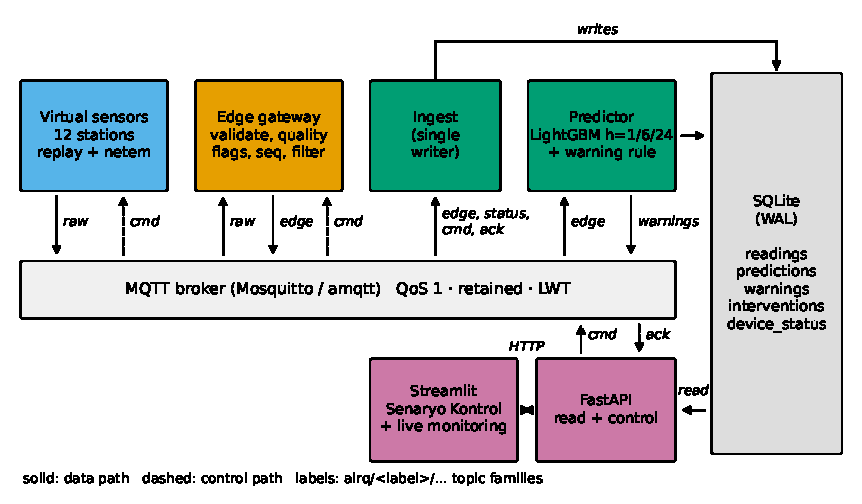
\includegraphics[width=0.85\textwidth]{figures/architecture.pdf}
\caption{Sistem mimarisi: sanal cihazlar ham telemetriyi MQTT'ye yayınlar; kenar geçidi doğrular; tek yazıcılı ingest SQLite'a yazar; tahmin servisi eğitimdeki özellik fonksiyonuyla 1, 6 ve 24 saat sonrasını tahmin edip uyarı üretir; FastAPI ve Streamlit panosu okur; komut kanalı (\texttt{cmd}/\texttt{ack}) aynı MQTT hattından cihazları ve kenarı yönetir.}
\label{fig:arch}
\end{figure*}

\textbf{Sanal cihazlar.} Gerçek kayıtlı ölçümler, her istasyon için ayrı bir MQTT istemcisi tarafından saat saat yayınlanır (\nSpeedSlow{}$\times$ hızda bir saniye bir simüle saattir). Her cihaz bir \emph{last will} (LWT) ile bağlanır; \texttt{online}/\texttt{offline} durumu retained olduğundan sonradan bağlanan da son durumu görür. Cihazın bir sıra numarası (\texttt{seq}) vardır, böylece kayıp ve tekrar tespit edilebilir. \emph{Neden:} fiziksel sensörümüz yok; ancak gerçek bir kentin gerçek kirlilik olaylarını canlı sistemden geçirebiliriz. Bu bir saha çalışması değil, iz sürümlü bir emülasyondur.

\textbf{MQTT ve QoS.} Haberleşme MQTT'dir. \emph{Neden:} sensörler için tasarlanmıştır, yayıncı ile abone birbirini tanımaz (yeni servis cihazlara dokunmadan eklenir) ve QoS, LWT ve retained mesaj gibi IoT'ye özgü özellikler hazırdır \cite{R7,R18,R19}. Telemetri QoS~1 ile gönderilir: kayıp tahmini bozacağından "en az bir kez" teslim seçilmiştir; bedeli olan tekrar, ingest'te \texttt{(istasyon, ts)} anahtarıyla idempotent kayıtla zararsız kılınır (Tablo~\ref{tab:topics}). Broker Mosquitto'dur (\nBrokerVersion{}); kurulu değilse saf-Python bir yedek (amqtt) kullanılır.

\begin{table}[t]
\caption{MQTT konuları, QoS ve retain bayrağı (\texttt{src/airq/iot/topics.py}).}
\label{tab:topics}
\centering\footnotesize
\begin{tabular}{llcc}
\toprule
Konu & Yayıncı $\rightarrow$ abone & QoS & Retain \\
\midrule
\texttt{airq/raw/\{st\}/telemetry} & cihaz $\rightarrow$ kenar & 1 & hayır \\
\texttt{airq/edge/\{st\}/telemetry} & kenar $\rightarrow$ ingest, tahmin & 1 & hayır \\
\texttt{airq/\{st\}/status} & cihaz (LWT) $\rightarrow$ ingest, tahmin & 1 & evet \\
\texttt{airq/\{st\}/heartbeat} & cihaz $\rightarrow$ (canlılık) & 0 & hayır \\
\texttt{airq/warnings/\{st\}} & tahmin $\rightarrow$ abone & 1 & hayır \\
\texttt{airq/cmd/\ldots} & API $\rightarrow$ cihaz, ağ, kenar & 1 & hayır \\
\texttt{airq/cmd/ack/\ldots} & uygulayan $\rightarrow$ denetleyici & 1 & hayır \\
\bottomrule
\end{tabular}
\end{table}

\textbf{Kenar katmanı.} Kenar geçidi her mesajı doğrular ve \pmtwo{} değerini beş kuralla işaretler: eksik, aralık dışı, ani sıçrama, takılı kalma ve \pmtwo{}$\le$PM$_{10}$ tutarlılığı; ayrıca mesaj düzeyinde \texttt{seq} boşluğu ve tekrar. Kenar filtresi \emph{açıkken} güvenilmez değer \texttt{null} ile değiştirilir. \emph{Neden:} bozuk bir değer tahmini bozar; kontrolü kaynağa yakın yapmak veriyi temizler ve hatalı cihazı erkenden görünür kılar \cite{R5,R21,R22}. Gerçek veride \pmtwo{}$>$PM$_{10}$ satırları \%\nPmInconsistentPct{} olduğundan katı kural çok yanlış alarm verirdi; tolerans eğitim verisinin uç değerlerinden seçilmiştir. Kural parametreleri yalnızca eğitim verisinden öğrenilir. Aynı kural tanımı hem çevrimdışı deneylerde (vektörel) hem canlı geçitte (artımlı) kullanılır; eşitlik bir testle denetlenir.

\textbf{Kayıt, tahmin ve arayüz.} Tek yazıcılı ingest, WAL kipindeki SQLite'a yazar. \emph{Neden:} şehir ağının yükü saatte \nDataStations{} satırdır; ayrı veritabanı sunucusu yerine SQLite yeterlidir (ölçek sınırı Bölüm~\ref{sec:limits}'de belirtilmiştir). Tahmin servisi her saatte diğer istasyonların ölçümünü en çok \nWaitMs{}~ms bekler, gelmeyen istasyon eksik sayılır. \emph{Neden:} aynı saatin mesajları karışık sırada gelir; beklemezsek komşu özellikleri rastgele eksik kalırdı, sonsuz beklersek çöken bir cihaz sistemi kilitlerdi. Tahmin servisi eğitimde kullanılan \texttt{build\_features} fonksiyonunu çalıştırır; bunun "çevrimdışı = çevrimiçi" olduğu, aynı verinin hem doğrudan hem MQTT hattından geçirilip özelliklerin ve tahminlerin eşit çıkmasıyla bir parite testinde doğrulanır. FastAPI salt-okunur uç noktalar ve kontrol uç noktaları sunar; Streamlit panosu yalnızca API'den okur.

\textbf{Senaryo Kontrol.} Panodan verilen müdahaleler (sensör değeri, hata türü, ağ koşulu, kenar filtresi) API'den MQTT komutlarına (\texttt{cmd}) dönüşür; her cihaz komutu uygular ve \texttt{ack} ile yanıtlar. Komutlar ve yanıtlar veritabanında kayıtlıdır. Bir puan tablosu, her müdahale için uyarının verilip verilmediğini, ne kadar önceden verildiğini ve tahminin ne kadar yanıldığını ölçer; referans değer cihazın söylediği değerden değil, \emph{komut kaydının cihazla aynı kodla yeniden oynatılmasından} üretilir. Yedi hazır senaryonun her birinin hipotezi çalıştırmadan önce yazılmıştır.

% ------------------------------------------------------------------------------------------------
\section{Yöntem}
\subsection{Veri}
Veri, UCI deposundaki Beijing Multi-Site Air-Quality veri setidir \cite{R8,R8d}: \nDataStations{} istasyon, istasyon başına \nDataHours{} saatlik kayıt (toplam \nDataRows{}), \nTrainStart{}'ten \nTestEnd{}'ye. \pmtwo{} değerlerinin \%\nDataMissingPct{}'i eksiktir; ortalama \nDataMean{}~\ugm{}, 95.\ yüzdelik \nDataPNinetyFive{}~\ugm{}'tür (Tablo~\ref{tab:dataset} Ek'te). Bu bir referans istasyon verisidir, düşük maliyetli sensör verisi değildir.

\subsection{Ön işleme ve sızıntı önlemleri}
Bölme kronolojiktir: eğitim \nTrainStart{}--\nTrainEnd{}, doğrulama \nValStart{}--\nValEnd{}, test \nTestStart{}--\nTestEnd{}. Tüm ölçekleme ve kural parametreleri yalnızca eğitim verisinde öğrenilir, tüm seçimler (hiperparametre, uyarı payı, aralık katsayısı) yalnızca doğrulamada yapılır, test dönemi her protokol için bir kez değerlendirilir. Eksik doldurma yalnızca geçmişe bakar (en çok 3 saat ileri doldurma); hedef zamanı sonraki bölmeye düşen satırlar atılır; hiçbir özellik $t$ anından sonraki bilgiyi kullanmaz ve $t{+}h$ anının PM$_{10}$ değeri hiçbir yerde yoktur \cite{R13,R16}. Bu önlemler birim testleriyle denetlenir.

\subsection{Özellikler ve modeller}
Özellikler: gecikmeli \pmtwo{} değerleri ve hareketli pencere istatistikleri, eşlik eden kirleticiler ve meteoroloji, takvim bileşenleri ve komşu istasyon özetleridir (ortalama, medyan, minimum, eğim, mevcut komşu sayısı). Komşular yalnızca eğitim verisinden belirlenir ve $k\in\{0,\nKThree{},\nKEleven{}\}$ olarak değiştirilir ($k{=}0$: komşu yok). Modeller: B0 persistence ($\hat y_{t+h}=y_t$), B1 mevsimsel naif (bir gün önceki aynı saat), B2 ridge ($k{=}0$), M1 LightGBM ($k{=}0$), M2a ($k{=}\nKThree{}$) ve M2b ($k{=}\nKEleven{}$) LightGBM \cite{R15}. LightGBM seçildi çünkü tablo özelliklerinde derin ağlarla rekabetçidir, eksik değerleri doğrudan işler ve SHAP ile açıklanabilir \cite{R26,R13,R14}; LSTM \cite{R9,R10} ve GNN \cite{R11,R12} daha fazla ayar gerektirir ve koordinat olmadan GNN'in avantajı sınırlıdır, açık komşu özellikleri ise hafif bir yaklaşıktır ve ablasyonla sınanır. Her ufuk ve $k$ için ayrı bir model, Optuna TPE ile doğrulama RMSE'si üzerinde, çalışma başına \nOptunaTrials{} deneme ile ayarlanır; modeller yalnızca eğitim verisiyle uydurulur ve LightGBM metin biçiminde, özellik listesi içeren bir manifestle saklanır.

\subsection{Erken uyarı}
$\theta\in\{\nThetaLow{},\nThetaHigh{}\}$~\ugm{} ve ufuk $h$ için uyarı kuralı $\hat y_{t+h}>\theta-\delta_{h,\theta}$'dır. Güvenlik payı $\delta$, doğrulamada F2 ($\beta{=}\nBeta{}$) en büyük olacak şekilde ızgaradan seçilir: erken uyarıda bir olayı kaçırmak, yanlış alarmdan daha pahalıdır ve $\delta$, modelin aşırı değerleri küçük tahmin etmesini telafi eder. Bir uyarı açıldıktan sonra aynı istasyon için \nCooldownH{} saat boyunca yeni uyarı verilmez. Aşım olayı, art arda en az 3 saat $\theta$'yı aşan bloktur; aralarında 6 saatten az olan bloklar birleştirilir ve başlangıç anı ilk saattir. \emph{Bölgesel haze} epizotu, en az 8 istasyonun $\theta{=}\nThetaHigh{}$'yi en az 6 saat aşmasıdır. Bir olay, başlangıcından önceki 24 saatte en az bir uyarı varsa "yakalanmış"tır; öncül süre başlangıç ile ilk uyarı arasındaki farktır. Bu basit tanım şişkin olabileceğinden (en basit yöntem bile yüksek yakalama gösterir) uyarının öngördüğü anın gerçekten olayın içine düştüğü \emph{ufukla eşleşen} tanım da raporlanır.

\subsection{Belirsizlik (RQ4)}
Her ufuk için $\alpha\in\{0.1,0.5,0.9\}$ quantile LightGBM modelleri eğitilir \cite{R27}; ham aralık $[q_{10},q_{90}]$ sıralanarak ($q_{10}\le q_{50}\le q_{90}$) elde edilir ve tek bir genişletme katsayısı $c$ yalnızca doğrulamada seçilir. Aralık tabanlı uyarı, nokta tahmin yerine $q_{90}$'a uygulanan aynı kuraldır ($\delta{=}0$). Test dönemine bakmadan önce protokol ve hipotez yazılıp sürüm kontrolüne eklenmiştir.

\subsection{RQ3 deney tasarımı}
\textbf{(a) Sistem ölçümü.} Her koşuda ayrı bir Mosquitto ve edge, ingest, tahmin ve cihaz filosu ayrı süreçler olarak çalışır. Sensörden kenara giden bağlantı uygulama katmanında emüle edilir (kayıp, gecikme, sıra bozulması; kaybolan mesaj hiç yayınlanmaz). Izgara: kayıp \%0/5/10/20, gecikme 0/200~ms, hız \nSpeedSlow{}$\times$ ve \nSpeedFast{}$\times$, ve \nSpeedFast{}$\times$ hızda 1/3/6 çevrimdışı cihaz; her yapılandırma \nReps{} tekrar (toplam \nRunsTotal{} koşu). \textbf{(b) Hatalı girdi.} Test girdilerine spike, stuck ve dropout enjekte edilir (tohumlu, hedef değerlere dokunulmaz) \cite{R21,R22}; aynı bozulma üzerinde kenar filtresi kapalı ve açık RMSE karşılaştırılır. Bu, arıza \emph{tespiti} başarısı iddiası değil, dayanıklılık ölçümüdür.

\subsection{Metrikler ve istatistik}
RMSE ana metriktir; MAE, $R^2$ ve sMAPE tablolarda bulunur. İyileşme persistence'a göre yüzde olarak verilir. Modeller arası fark, istasyon başına Diebold--Mariano testiyle \cite{R24,R25}, 12 istasyon için Holm düzeltmesiyle sınanır; güven aralıkları 24 saatlik bloklarla bootstrap'tan gelir. Özellik katkısı SHAP ile \cite{R26} ve ablasyon sonuçlarıyla birlikte yorumlanır.

% ------------------------------------------------------------------------------------------------
\section{Deney Kurulumu}
Tohum \nSeed{} sabittir; LightGBM deterministik kipte çalışır. Tüm ölçümler tek bir Windows bilgisayarda alınmıştır (\nCpuCount{} mantıksal çekirdek, \nRamGb{}~GB RAM, Python~\nPyVersion{}); mutlak süreler bu makineye özgüdür, bu yüzden bağıl etkiler vurgulanır. Hiperparametre araması çalışma başına \nOptunaTrials{} denemedir. Canlı sistem ölçümleri Bölüm~\ref{sec:rq3a}'da anlatılan ızgarayla \nSimDays{} simüle gün üzerinde çalıştırılmıştır.

% ------------------------------------------------------------------------------------------------
\section{Bulgular}
Ondalık ayırıcı nokta ile gösterilmiştir. Her sayı \texttt{reports/} altındaki bir dosyadan üretilir (\texttt{paper/NUMBERS.md}).

\subsection{RQ1: tahmin doğruluğu}
Tablo~\ref{tab:rq1_main}, test yılının sonuçlarını verir. LightGBM ve ridge, persistence'tan istatistiksel olarak anlamlı biçimde iyidir: M2b, 1, 6 ve 24 saatte sırasıyla \nDmMtwobVsBZeroHOne{}, \nDmMtwobVsBZeroHSix{} ve \nDmMtwobVsBZeroHTwentyFour{} istasyonda anlamlıdır (toplam \nLosoStations{}; Holm düzeltmeli DM). Mevsimsel naif model hiçbir istasyonda persistence'ı geçmez. Kazanç ufukla artar: M2b persistence'a göre \%\nImprMtwobHOne{} (1 sa), \%\nImprMtwobHSix{} (6 sa) ve \%\nImprMtwobHTwentyFour{} (24 sa) daha düşük RMSE verir (Şekil~\ref{fig:horizon}).

\widetable{rq1_main}

\begin{figure}[t]
\centering
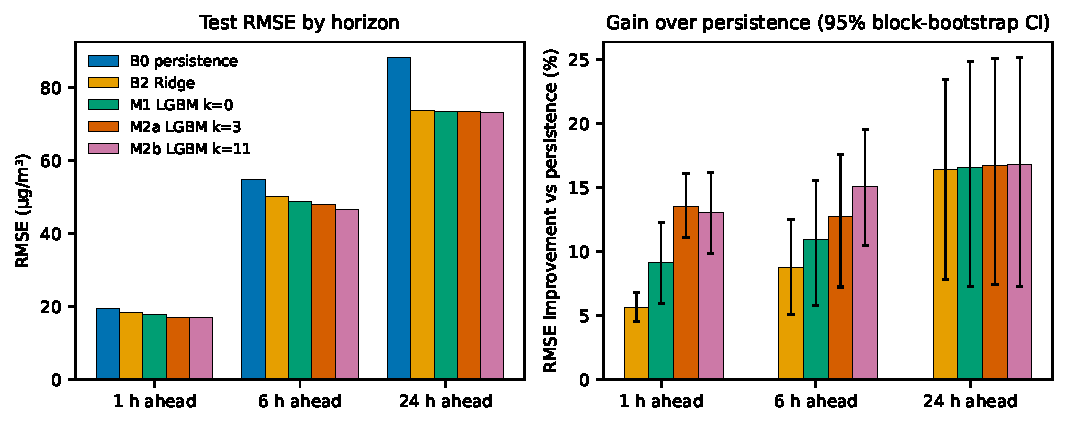
\includegraphics[width=\columnwidth]{figures/rq1_horizon.pdf}
\caption{Ufuk bazında test RMSE'si ve persistence'a göre iyileşme.}
\label{fig:horizon}
\end{figure}

\textbf{Komşu istasyonların katkısı.} Tek-istasyon LightGBM'e göre \nKEleven{} komşu, RMSE'yi 1 saatte \%\nAblKelevenHOne{} (\nAblKelevenSigHOne{} istasyonda anlamlı), 6 saatte \%\nAblKelevenHSix{} (\nAblKelevenSigHSix{}) düşürür; 24 saatte fark \%\nAblKelevenHTwentyFour{}'tür (\nAblKelevenSigHTwentyFour{} istasyonda anlamlı). Yakın istasyonlar kısa menzilli bilgi (yaklaşan kirlilik) taşır, ertesi güne ait bilgi taşımaz (Şekil~\ref{fig:ablation}). SHAP ile en etkili özellik güncel \pmtwo{} değeridir (ortalama $|$SHAP$|$: \nShapLagZeroHOne{} 1 saatte, \nShapLagZeroHSix{} 6 saatte, \nShapLagZeroHTwentyFour{} 24 saatte); komşu ortalaması 6 saatte \nShapNbMeanHSix{} ile ikinci sıradadır.

\begin{figure}[t]
\centering
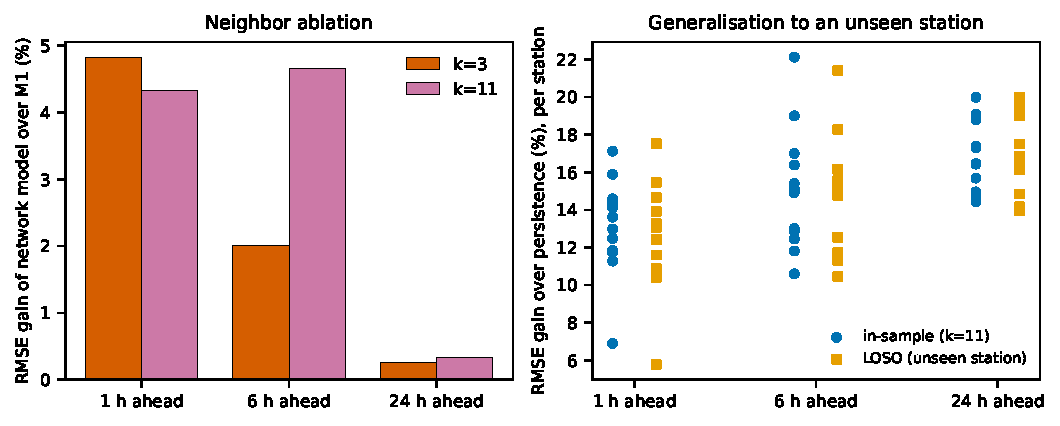
\includegraphics[width=\columnwidth]{figures/rq1_ablation_loso.pdf}
\caption{Komşu ablasyonu ve görülmemiş istasyon (LOSO) sonuçları.}
\label{fig:ablation}
\end{figure}

\textbf{Görülmemiş istasyon.} Bir istasyon eğitimden tamamen çıkarıldığında persistence'a göre ortalama iyileşme \%\nLosoMeanHOne{}, \%\nLosoMeanHSix{}, \%\nLosoMeanHTwentyFour{}'tür (1, 6, 24 sa); istasyon eğitimdeyken \%\nLosoInSampleHOne{}, \%\nLosoInSampleHSix{}, \%\nLosoInSampleHTwentyFour{}. Model, \nLosoBetterHOne{}/\nLosoStations{} istasyonda her ufukta persistence'ı geçer; yani genelleme ihmal edilebilir kayıpla korunur.

\textbf{Olumsuz sonuç: aşırı olaylar.} Hedefi eğitim 95.\ yüzdeliğinin (\nExtPNinetyFive{}~\ugm{}) üzerinde olan satırlarda M2b, persistence'ı geçmez: RMSE 1 saatte \nExtRmseMtwobHOne{} (persistence \nExtRmsePersistHOne{}), 6 saatte \nExtRmseMtwobHSix{} (\nExtRmsePersistHSix{}), 24 saatte \nExtRmseMtwobHTwentyFour{} (\nExtRmsePersistHTwentyFour{}). Ortalama hata (gerçek eksi tahmin) pozitiftir: M2b düşük tahmin eder (\nExtBiasMtwobHOne{}, \nExtBiasMtwobHSix{} ve \nExtBiasMtwobHTwentyFour{}~\ugm{}). Kare hata amacı ortalamaya çeker; tepe saatleri ise uyarılar için en önemlileridir.

\subsection{RQ2: erken uyarı}
Test yılında \nThetaHigh{}~\ugm{} üzerinde \nEventsHundred{} aşım olayı ve \nEventsHaze{} bölgesel haze epizotu vardır. Tablo~\ref{tab:rq2_warning}'de M2b'nin uyarı başarımı görülür: F2, 1 saatte \nWarnFtwoMtwobHOne{} (precision \nWarnPrecMtwobHOne{}, recall \nWarnRecMtwobHOne{}), 6 saatte \nWarnFtwoMtwobHSix{}, 24 saatte \nWarnFtwoMtwobHTwentyFour{}'dür. Olay yakalama oranı \nWarnEvRecMtwobHOne{} (1 sa), \nWarnEvRecMtwobHSix{} (6 sa), \nWarnEvRecMtwobHTwentyFour{} (24 sa); yanlış alarm oranı \nWarnFaMtwobHOne{}, \nWarnFaMtwobHSix{}, \nWarnFaMtwobHTwentyFour{}'tür. 1 ve 6 saatte öğrenilmiş model, persistence'tan biraz daha yüksek F2 ve daha az yanlış alarm verir (1 saatte \nWarnFaMtwobHOne{} karşı \nWarnFaPersistHOne{}). Medyan öncül süre 1, 6 ve 24 saatte \nWarnLeadMtwobHOne{}, \nWarnLeadMtwobHSix{} ve \nWarnLeadMtwobHTwentyFour{} saattir; ufukla eşleşen olay yakalama \nWarnMEvRecMtwobHOne{}, \nWarnMEvRecMtwobHSix{} ve \nWarnMEvRecMtwobHTwentyFour{}'tür.

\textbf{Olumsuz sonuç: 24 saat.} 24 saatte persistence daha yüksek F2'ye (\nWarnFtwoPersistHTwentyFour{} karşı \nWarnFtwoMtwobHTwentyFour{}) ve tüm olayları yakalayan bir recall'a (\nWarnEvRecPersistHTwentyFour{}) sahiptir. Bölgesel haze epizotlarında M2b 24 saatte \nHazeCaughtMtwobHTwentyFour{} epizodu yakalar, persistence \nHazeCaughtPersistHTwentyFour{}'ünü (Şekil~\ref{fig:haze} bir epizodu gösterir). Bu, RQ1'deki tepe değerleri düşük tahmin etme bulgusuyla tutarlıdır; nedeni ayrıca izole etmedik.

\widetable{rq2_warning}

\begin{figure}[t]
\centering
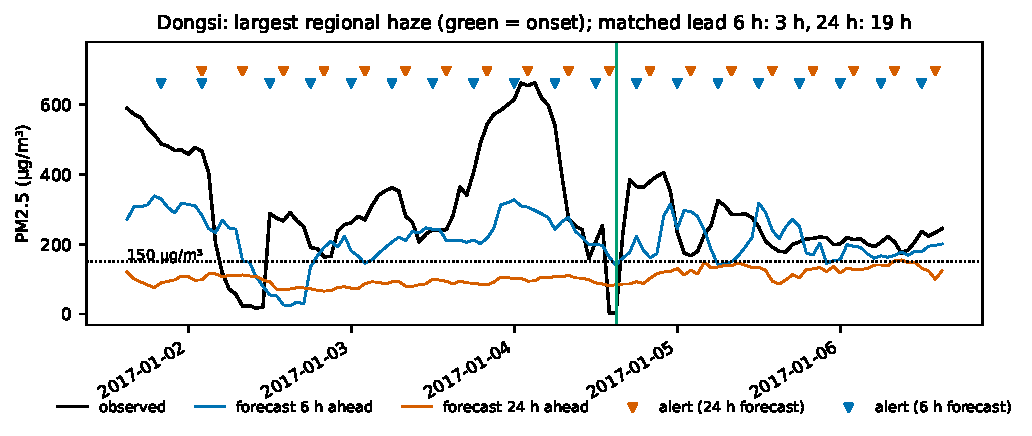
\includegraphics[width=\columnwidth]{figures/rq2_haze_example.pdf}
\caption{Bir haze epizodunda gerçek değer, tahmin ve uyarılar.}
\label{fig:haze}
\end{figure}

\subsection{RQ3a: ağ bozulması altında sistem}\label{sec:rq3a}
Tablo~\ref{tab:rq3a} ve Şekil~\ref{fig:rq3a}, \nReps{} tekrarlı tam ızgarayı özetler. Teslim oranı yapılandırılan kayıpla örtüşür: \%5, \%10 ve \%20 kayıpta sırasıyla \nPdrFive{}, \nPdrTen{}, \nPdrTwenty{}; tekrar oranı sıfırdır. Cihazdan veritabanına medyan gecikme gecikmesiz \nLatDbMedian{}~ms, 200~ms emülasyonla \nLatDbMedianDelay{}~ms'dir. Tahmin zararı (eşleştirilmiş 1 saatlik RMSE artışı, \nReps{} tekrar ortalaması) \%5 kayıpta \nDmgFive{}, \%10 kayıpta \nDmgTen{} ve \%20 kayıpta \nDmgTwenty{}~$\pm$~\nDmgTwentyStd{}~\ugm{}'dür; 6 ve 24 saatte değişim gürültü içindedir. 200~ms gecikme hiçbir tahmini değiştirmez (\nWaitMs{}~ms bekleme süresinden kısadır).

\textbf{Gerçek zaman payı.} \nSpeedSlow{}$\times$ hızda tahmin servisi kayıpsız ve çoğunlukla \%5--10 kayıpta yetişir (medyan uyarı gecikmesi \nWarnLatKeepUp{}~s); fakat \%20 kayıpta \nRunsTwenty{} koşunun \nBehindTwenty{}'ünde ve \%5 kayıpta \nRunsFive{} koşunun \nBehindFive{}'inde geride kalarak medyan \nWarnLatBehind{}~s gecikmeye ulaşır. Neden, kayıp saatlerde eksik bir istasyon için \nWaitMs{}~ms beklemenin, saat başına bir saniyelik bütçeyi tüketmesidir.

\textbf{Ölçümün bulduğu kusur ve düzeltmesi.} Aynı bekleme, kalıcı olarak çevrimdışı bir cihazın \emph{her saat} \nWaitMs{}~ms boşa beklemeye yol açması anlamına geliyordu: \nSpeedFast{}$\times$ hızda tam ağda medyan uyarı gecikmesi \nOffLatFullBefore{}~s iken bir çevrimdışı cihazla \nOffLatOneBefore{}~s oldu. Tahmin servisi artık, retained durumu \texttt{offline} olan istasyonu kısa bir ek süreden sonra beklemez (durum mesajı, kenardan geçen son ölçümlerin önüne geçebildiğinden ek süre gereklidir). Son kodla yeniden ölçümde bir çevrimdışı cihazla gecikme \nOffLatOneAfter{}~s (tam ağda \nOffLatFullAfter{}~s), üç ve altı cihazla \nOffLatThreeAfter{} ve \nOffLatSixAfter{}~s'tir; hiçbir koşu geride kalmadı, tahmin kalitesi değişmedi. Düzeltme \emph{mesaj kaybında} yardımcı olmaz: kaybolan mesaj hiçbir şey duyurmaz, bu yüzden o bekleme sürer.

\widetable{rq3a}

\begin{figure}[t]
\centering
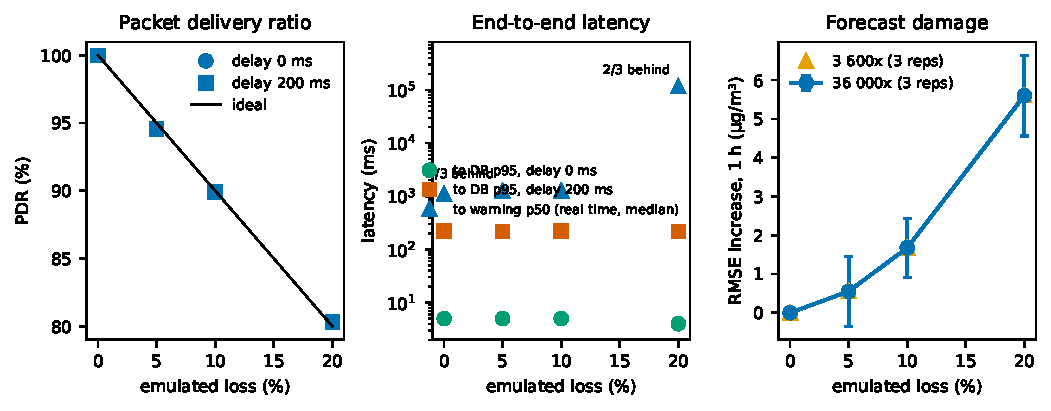
\includegraphics[width=\columnwidth]{figures/rq3a_system.pdf}
\caption{Kayıp oranına göre teslim oranı, uyarı gecikmesi ve tahmin zararı.}
\label{fig:rq3a}
\end{figure}

\subsection{RQ3b: hatalı sensör girdisi}
Hatalı girdinin, son 24 saatinde hata içeren satırlardaki RMSE artışı Tablo~\ref{tab:rq3b}'de ve Şekil~\ref{fig:rq3b}'dedir. 1 saatte persistence'ın zararı \nRobOffPersistHOne{}~\ugm{}'den \nRobOnPersistHOne{}'ye iner (\%\nRobRecPersistHOne{} geri kazanım); M2b'de zarar \nRobOffMtwobHOne{}'den \nRobOnMtwobHOne{}'ye iner (\%\nRobRecMtwobHOne{}). Komşu özellikli model, hatalı kendi sensörüne karşı daha dayanıklıdır (zarar \nRobOffMtwobHOne{} karşı tek-istasyon LightGBM'in \nRobOffMoneHOne{}'i). Hata en çok 1 saatte, en az 24 saatte zarar verir (M2b: \nRobOffMtwobHTwentyFour{}~\ugm{}). \textbf{Filtre basit modele çok, öğrenilmiş modele daha az yardım eder;} nedenini sınamadık, bir olasılık filtrenin değeri \emph{eksik} yaparak modelin kullanabileceği bilgiyi kaldırmasıdır.

\begin{table}[t]
\caption{Hatalı girdinin RMSE'ye etkisi, kenar filtresi kapalı ve açık (seçilmiş satırlar; tam tablo \texttt{reports/tables/rq3b\_robustness.csv}).}
\label{tab:rq3b}
\centering\footnotesize
\begin{tabular}{llrrrr}
\toprule
Model & $h$ & Temiz & Zarar, kapalı & Zarar, açık & Geri (\%) \\
\midrule
B0 & 1 & \nRobCleanPersistHOne{} & \nRobOffPersistHOne{} & \nRobOnPersistHOne{} & \nRobRecPersistHOne{} \\
M1 & 1 & \nRobCleanMoneHOne{} & \nRobOffMoneHOne{} & \nRobOnMoneHOne{} & \nRobRecMoneHOne{} \\
M2b & 1 & \nRobCleanMtwobHOne{} & \nRobOffMtwobHOne{} & \nRobOnMtwobHOne{} & \nRobRecMtwobHOne{} \\
M2b & 6 & \nRobCleanMtwobHSix{} & \nRobOffMtwobHSix{} & \nRobOnMtwobHSix{} & \nRobRecMtwobHSix{} \\
\bottomrule
\end{tabular}
\end{table}

\begin{figure}[t]
\centering
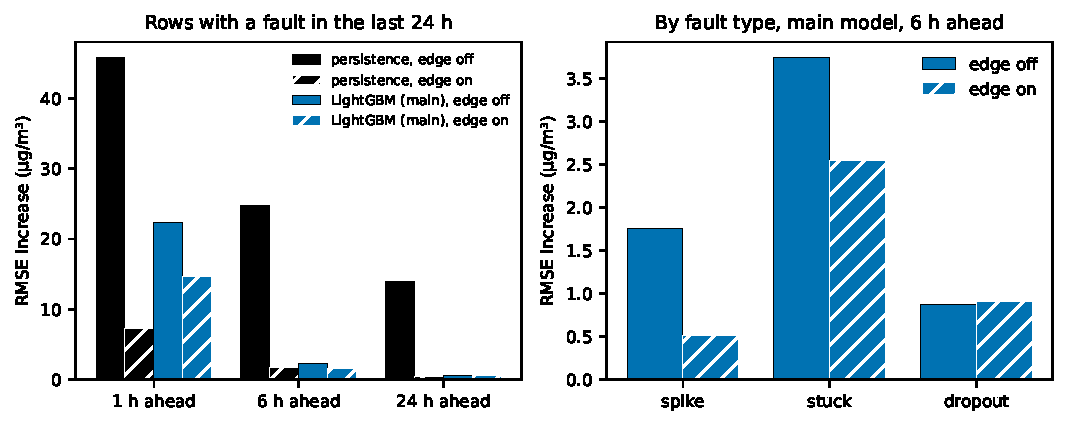
\includegraphics[width=\columnwidth]{figures/rq3b_damage.pdf}
\caption{Hata türüne göre RMSE artışı, kenar filtresi kapalı ve açık.}
\label{fig:rq3b}
\end{figure}

\subsection{Senaryo Kontrol}
Yedi senaryo birer kez çalıştırılmış, beklenen sonuç çalıştırmadan önce yazılmıştır: \nScnTotal{} kontrolün \nScnConfirmed{}'i doğrulanmış, \nScnRefuted{}'i çürütülmüştür (kenar filtresi kapalı takılı kalan bir sensörün sonraki 6 saatte 6 saatlik MAE'yi \nScnStuckReference{}~\ugm{}'in üzerine çıkarması beklenmişti; ölçülen \nScnStuckMeasured{}~\ugm{} oldu). Ağ bozulması senaryosunda teslim oranı \nScnDelivery{}, p95 gecikme \nScnLatencyP{}~ms; gerçek haze yeniden oynatmasında uyarı \nScnHazeLead{} saat önceden verilmiştir.

Eşleştirilmiş çalıştırmalar aynı arıza penceresini filtre kapalı ve açık iki kez oynatır (\nAbSpikeWindows{} başlangıç tarihi). Spike altında filtre 1 saatlik MAE'yi ortalama \nAbSpikeGainHOne{}~\ugm{} düşürür (\nAbSpikeWins{}/\nAbSpikeWindows{} pencerede yardımcı), ancak 6 saatlik hatayı \nAbSpikeGainHSix{}~\ugm{} değiştirir (negatif: zarar). Takılı kalma altında filtre 1 saatte hafif zararlıdır (\nAbStuckGainHOne{}) ve 6 saatte nötrdür (\nAbStuckGainHSix{}). Pencere sayısı küçüktür; bunlar istatistik değil gösterimdir.

\subsection{RQ4: belirsizlik}
Ham $[q_{10},q_{90}]$ aralığının kapsaması hedef 0.80'in altındadır (\nCovRawHOne{}, \nCovRawHSix{}, \nCovRawHTwentyFour{}); doğrulamada seçilen genişletme katsayısı $c{=}\nFactorHOne{}$, \nFactorHSix{}, \nFactorHTwentyFour{} ile kapsama \nCovCalHOne{}, \nCovCalHSix{} ve \nCovCalHTwentyFour{}'e çıkar (Tablo~\ref{tab:rq4_coverage}, Şekil~\ref{fig:rq4}). Kapsama \emph{koşullu} değildir: aşırı hedeflerde \nCovExtCalHOne{}, \nCovExtCalHSix{} ve \nCovExtCalHTwentyFour{}'e düşer. Tek bir sayı, düşük tahmin eden modeli düzeltemez. $q_{90}$ tabanlı uyarı, noktasal uyarıya göre bir recall--precision takasıdır (Tablo~\ref{tab:rq4_warning}): 24 saatte recall \nQwRecMtwobHTwentyFour{}'den \nQwRecQnineHTwentyFour{}'e, F2 \nQwFtwoMtwobHTwentyFour{}'den \nQwFtwoQnineHTwentyFour{}'e çıkar; yanlış alarm \nQwFaMtwobHTwentyFour{}'den \nQwFaQnineHTwentyFour{}'e yükselir. 1 saatte kazanç yoktur (F2 \nQwFtwoQnineHOne{} karşı \nQwFtwoMtwobHOne{}).

\begin{figure}[t]
\centering
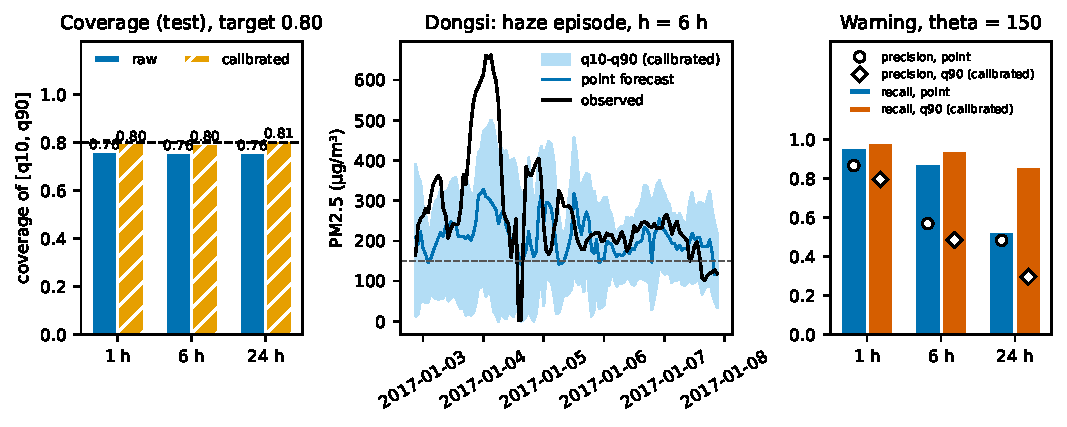
\includegraphics[width=\columnwidth]{figures/rq4_uncertainty.pdf}
\caption{Kapsama ve aralık genişliği; $q_{90}$ tabanlı uyarı.}
\label{fig:rq4}
\end{figure}

\widetable{rq4_coverage}
\widetable{rq4_warning}

% ------------------------------------------------------------------------------------------------
\section{Tartışma}
\textbf{Komşu bilgisinin değeri ufka bağlıdır.} Komşu istasyonlar 1 ve 6 saatte tek-istasyon modele göre anlamlı kazanç sağlar, 24 saatte sağlamaz. Bu, kirlilik dalgasının şehirde yayılmasının kısa menzilde ölçülebilir bilgi taşıdığını, uzun menzilde meteorolojik rejimin baskın olduğunu düşündürür; bunu ayrıca sınamadık. Bu bulgu, bir ağdaki cihazların birbirini görmesinin \emph{yalnızca} erken ufuklarda işe yaradığını ve uzun ufuk için başka bilgi (hava durumu tahmini) gerektiğini gösterir.

\textbf{Aşırı olaylarda persistence'tan geri kalmak.} En çok önem taşıyan tepe saatlerinde öğrenilmiş model persistence'ı geçmez ve düşük tahmin eder; bu, 24 saatte uyarı recall'unu da düşürür. $q_{90}$ tabanlı uyarı recall'u artırır ancak yanlış alarm bedeliyle; kapsama aşırı hedeflerde düşük kalır. Pratik sonuç: nokta tahmin 1 ve 6 saatte güvenilir bir uyarı temelidir; 24 saatte ihtiyatlı (üst sınır) kural ya da farklı bir amaç fonksiyonu gerekir.

\textbf{Ağ ve veri kalitesi.} Kayıp, tahmini birinci derecede bozmaz (20\% kayıpta 1 saatte yaklaşık \nDmgTwenty{}~\ugm{}), ama \emph{gerçek zamanlı} servisin tasarımını sınar: bekleme süresi gibi bir tasarım seçimi, kayıp ve çevrimdışı cihaz altında sistemin yetişip yetişmediğini belirler. Bunu ancak sistemi ağ koşullarıyla birlikte ölçmek ortaya çıkarabildi.

\textbf{Kenar doğrulamasının rolü.} Filtre, basit modelde zararın büyük kısmını geri alır, öğrenilmiş modelde daha azını; eşleştirilmiş koşularda ise spike altında 1 saatte yardım eder, 6 saatte zarar verebilir. Yani kenar doğrulaması tek başına bir kazanç değildir; hangi modelle ve hangi ufukla birlikte kullanıldığına bağlıdır.

% ------------------------------------------------------------------------------------------------
\section{Sınırlamalar ve Geçerlilik Tehditleri}\label{sec:limits}
(1) \textbf{İz sürümlü emülasyon:} gerçek kayıtlı ölçümler yeniden oynatılır; saha çalışması değildir. (2) \textbf{Referans istasyon verisi:} düşük maliyetli sensörler kayar ve neme duyarlıdır \cite{R1,R20}; saha davranışı farklı olacaktır. (3) \textbf{Sentetik hatalı girdi:} hata türleri enjekte edilmiştir. (4) \textbf{Tek şehir ve tek test yılı.} (5) \textbf{Uygulama katmanında ağ emülasyonu:} kaybolan mesaj yayınlanmaz; MQTT yeniden iletimi ve TCP kuyruk gecikmesi ölçülmemiştir. (6) \textbf{Güvenlik yok:} komut kanalı kimlik doğrulamasızdır ve yalnızca yerel ağ içindir; gerçek dağıtım TLS ve erişim denetimi gerektirir. (7) \textbf{Tek makine:} mutlak süreler makineye özgüdür; canlı senaryolar birer kez, eşleştirilmiş çalıştırmalar \nAbSpikeWindows{} pencereyle yapılmıştır. (8) SQLite tek yazıcılı küçük yük için uygundur; büyük ağlar için ölçeklenmez. (9) Karşılaştırma için dayandığımız bir kaynak (\cite{R13}) hakemli sürümü olmayan bir ön baskıdır.

% ------------------------------------------------------------------------------------------------
\section{Sonuç ve Gelecek Çalışmalar}
Gerçek bir kentsel ağın kayıtlı verisiyle MQTT, kenar doğrulaması, SQLite, LightGBM ve canlı bir pano içeren uçtan uca bir sistem kurduk ve tahmin ile erken uyarının, ölçümü taşıyan IoT hattıyla birlikte ölçülebileceğini gösterdik. Komşu özellikli LightGBM persistence'a göre 1, 6 ve 24 saatte \%\nImprMtwobHOne{}, \%\nImprMtwobHSix{} ve \%\nImprMtwobHTwentyFour{} iyileşme sağlar; erken uyarı 1 ve 6 saatte işe yarar, 24 saatte yetersizdir; kayıp ve çevrimdışı cihaz tahmin servisinin gerçek zaman davranışını belirler ve ölçüm bir tasarım kusurunu açığa çıkarmıştır; kenar doğrulaması hatalı girdinin zararını modele ve ufka bağlı olarak azaltır.

Gelecek çalışma: gerçek düşük maliyetli sensörlerle (örneğin PMS5003 ve ESP32) saha testi ve kalibrasyon \cite{R20,R1}; TLS ve erişim denetimi; grafik sinir ağları \cite{R12}; kenarda tahmin \cite{R6}; aşırı olaylar için asimetrik amaç fonksiyonları; ayrı bir anomali tespiti modülü.

\textbf{Erişilebilirlik.} Kod, sonuç tabloları ve sürüm notları \url{https://github.com/furkantopcuu/airq-iot} adresindedir; \texttt{python -m scripts.run_all} ham veriden tüm sonuçları yeniden üretir; paketlenmiş eğitimli modeller ve kayıtlı bir demo koşusu depo sürümünde sağlama toplamlarıyla yayımlanmıştır.

\bibliographystyle{IEEEtran}
\bibliography{refs}

\appendices
\section{Veri Seti Özeti}
\widetable{dataset}

\end{document}
